\subsection{Detailed Examples\label{sec:detailedex}}

Below are six examples, each followed by output generated to demonstrate how
to use the functions in the package: 
\begin{itemize}
\item Example~1 shows the calculation of
information ratios and boundaries based on default values for
\texttt{gsDesign()}. This also demonstrates the difference in sample size when
assuming binding versus non-binding (the default) lower bounds. 
\item Example~2 demonstrates two-sided testing and user-specified spending; 
commands demonstrating O'Brien-Fleming, Pocock and Wang-Tsiatis bounds are also shown.
\item Example~3 demonstrates use of the logistic spending function. It also 
gives further comments on the other two-parameter spending functions as 
well as the three-parameter t-distribution spending function. 
\item Example~4 shows how to use \texttt{gsProbability()} to calculate 
boundary crossing probabilities. 
\item Example~5 demonstrates how to design a non-inferiority study. 
\item Example~6 demonstrates a non-inferiority study that also evaluates 
superiority.
\end{itemize}

\subsection*{Example 1: Default input and standard spending functions}

For this example, we begin by noting some defaults for \texttt{gsDesign()},
and continue with the default call and its associated standard print and plot
output. Next, we show the structure of information returned by
\texttt{gsDesign()}. Since the defaults provide sample size ratios for a group
sequential design compared to a design with no interim analysis, we
demonstrate how to generate sample sizes for a binomial trial with a binomial
endpoint. Finally, we demonstrate some standard spending functions and how to
set their corresponding parameters.

\bigskip

The main parameter defaults that you need to know about are as follows:

\begin{enumerate}
\item Overall Type I error $\alpha = 0.025$ (one-sided)

\item Overall Type II error $\beta = 0.1$ (Power = $90\%$)

\item Two interim analyses plus the final analysis (\texttt{k=3})

\item Asymmetric boundaries, which means we may stop the trial for futility or
superiority at an interim analysis.

\item $\beta$-spending is used to set the lower stopping
boundary. This means that the spending function controls the incremental
amount of Type II error at each analysis.

\item Non-binding lower bound. Lower bounds are sometimes considered as
guidelines, which may be ignored during the course of the trial. Since Type I
error is inflated if this is the case, regulators often demand that the lower
bounds be ignored when computing Type I error.

\item Hwang-Shih-DeCani spending functions with $\gamma = -4$ for the upper
bound and $\gamma = -2$ for the lower bound. This provides a conservative,
O'Brien-Fleming-like superiority bound and a less conservative lower bound.
\end{enumerate}

We begin with the call 
\verb!x <- gsDesign()!
to generate a design using all default arguments. The next line
prints a summary of \texttt{x}; this produces the same effect as
\texttt{print(x)} or \texttt{print.gsDesign(x)}. Note that while the total
Type I error is $0.025$, this assumes the lower bound is ignored if it is
crossed; looking lower in the output we see the total probability of crossing
the upper boundary at any analysis when the lower bound stops the trial is
$0.0233$. Had the option 
\verb!x <- gsDesign(test.type=3)!
been run, both of these numbers would assume the trial
stops if the lower bound stopped and thus would both be $0.025$. Next, a
boundary plot is generated using \texttt{plot(x)}. A power plot is generated
with the statement \texttt{plot(x, plottype = 2)}. The solid lines in this plot
are, in ascending order, the cumulative power of the design first and second
interims and final analysis, respectively, for different values of
$\theta/\delta$, where $\delta$ is the standardized treatment effect for which
the trial is powered and $\theta$ is the true/underlying standardized
treatment effect. The dashed lines, in descending order, are one minus the
probability of crossing the lower boundary for the first and second interims, respectively.

\bigskip

\begin{verbatim}
> x <- gsDesign()
> x
Asymmetric two-sided group sequential design with 90 % power and 2.5 % Type I Error.
Upper bound spending computations assume trial continues if lower bound is crossed.

           Sample
            Size    ----Lower bounds----  ----Upper bounds-----
  Analysis Ratio*   Z   Nominal p Spend+  Z   Nominal p Spend++
         1  0.357 -0.24    0.4057 0.0148 3.01    0.0013  0.0013
         2  0.713  0.94    0.8267 0.0289 2.55    0.0054  0.0049
         3  1.070  2.00    0.9772 0.0563 2.00    0.0228  0.0188
     Total                        0.1000                 0.0250 
+ lower bound beta spending (under H1): Hwang-Shih-DeCani spending function with gamma = -2
++ alpha spending: Hwang-Shih-DeCani spending function with gamma = -4
* Sample size ratio compared to fixed non-group sequential design

Boundary crossing probabilities and expected sample size assuming any cross stops the trial

Upper boundary (power or Type I Error)
          Analysis
   Theta      1      2      3  Total   E{N}
  0.0000 0.0013 0.0049 0.0171 0.0233 0.6249
  3.2415 0.1412 0.4403 0.3185 0.9000 0.7913

Lower boundary (futility or Type II Error)
          Analysis
   Theta      1      2      3  Total
  0.0000 0.4057 0.4290 0.1420 0.9767
  3.2415 0.0148 0.0289 0.0563 0.1000

> plot(x)
> plot(x, plottype=2)
\end{verbatim}
\begin{figure}
\begin{center}
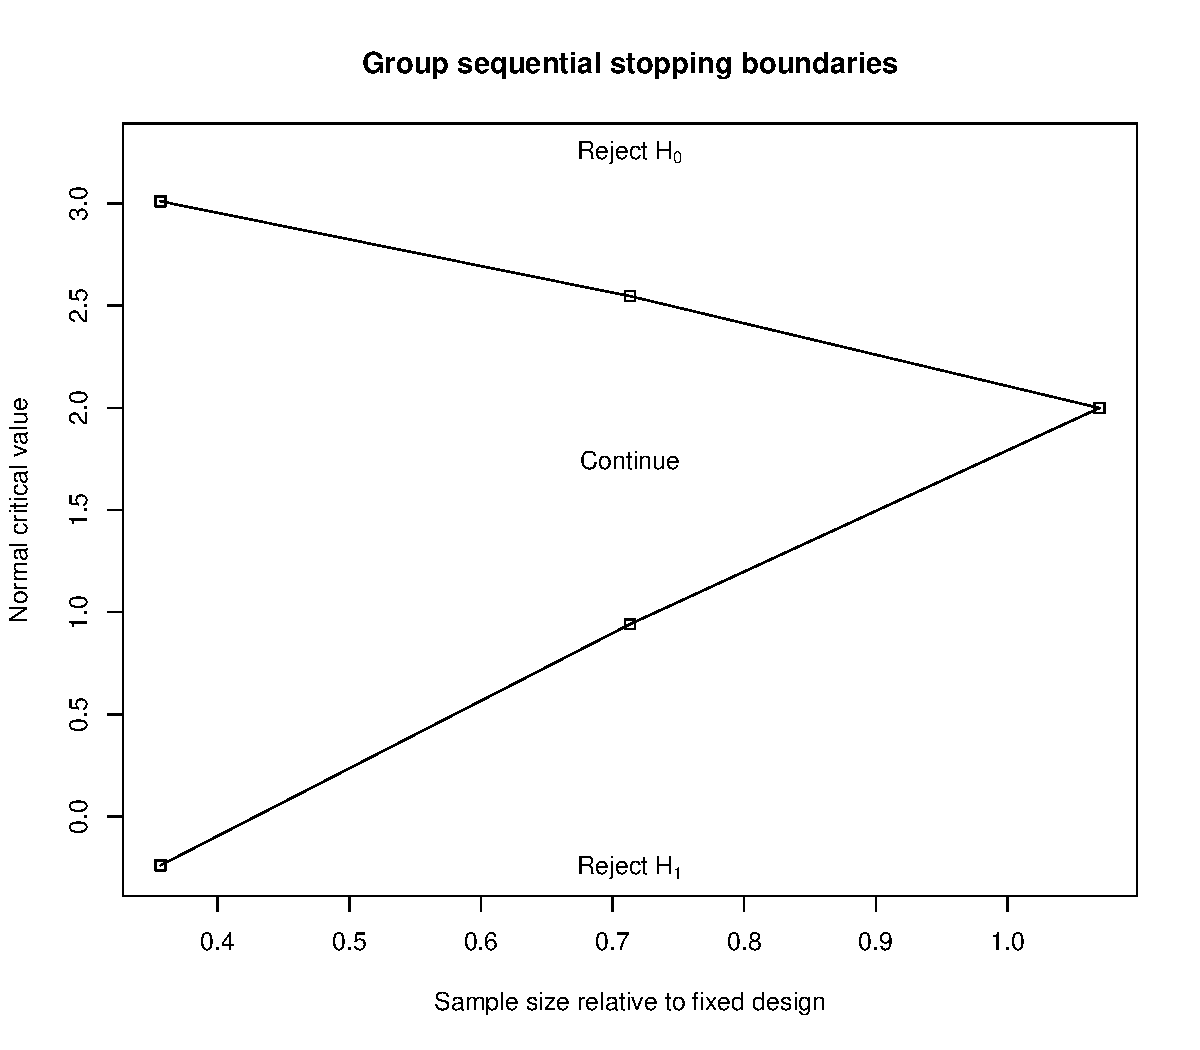
\includegraphics[width=.6\textwidth]{figs/boundplot.pdf}
\end{center}
\caption{Default plot for gsDesign object from example 1}
%RBC plot needs updating
\end{figure}%

\begin{figure}
\begin{center}
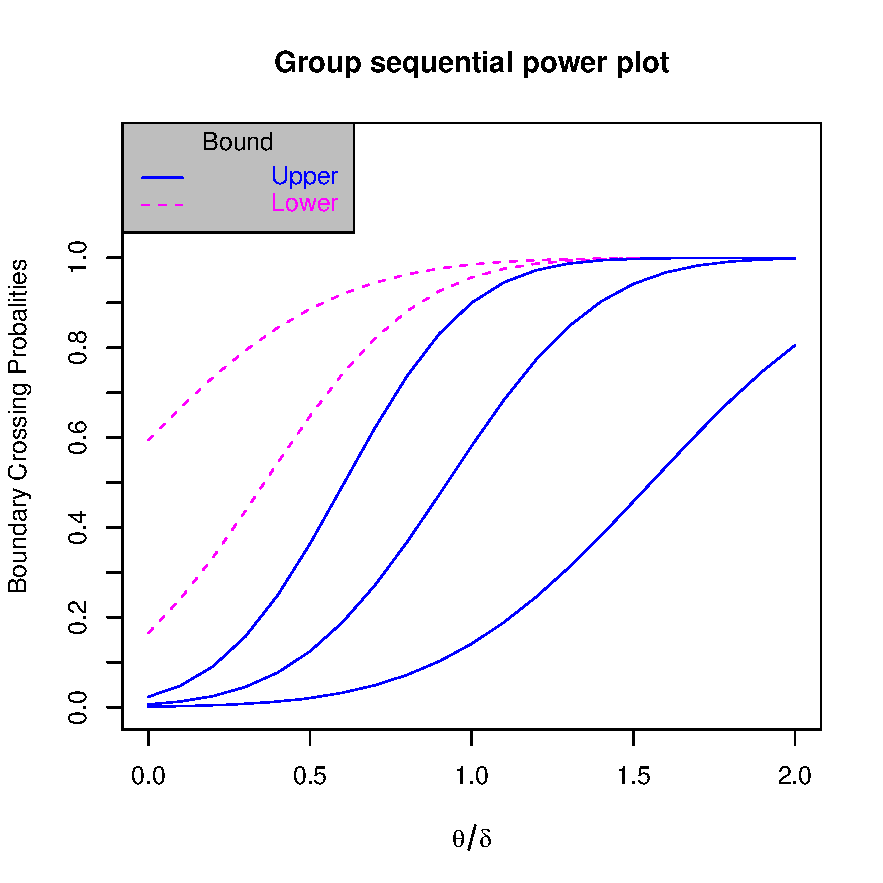
\includegraphics[width=.6\textwidth]{figs/powerplot.pdf}
\end{center}
\caption{Power plot (plottype=2) for gsDesign object from example 1}
\end{figure}%


\bigskip

Above we have seen standard output for \texttt{gsDesign()}. Now we look at how
to access individual items of information about what is returned from
\texttt{gsDesign()}. First, we use \texttt{summary(x)} to list the elements of
\texttt{x}. To view an individual element of \texttt{x}, we provide the
example \texttt{x\$delta}. See Section~\ref{sec:statmethods}, Statistical Methods, for an explanation of this value of \texttt{x\$delta}. Other elements of 
\texttt{x} can be accessed in the same way. Of particular interest are the 
elements \texttt{upper} and \texttt{lower}. These are both objects containing 
multiple variables concerning the upper and lower boundaries and boundary 
crossing probabilities.
The command summary \texttt{x\$upper} shows what these variables are. 
The upper boundary is shown with the command \texttt{x\$upper\$bound}.

\bigskip

\begin{verbatim}
> summary(x)
           Length Class   Mode     
k          1      -none-  numeric  
test.type  1      -none-  numeric  
alpha      1      -none-  numeric  
beta       1      -none-  numeric  
astar      1      -none-  numeric  
delta      1      -none-  numeric  
n.fix      1      -none-  numeric  
timing     3      -none-  numeric  
tol        1      -none-  numeric  
r          1      -none-  numeric  
n.I        3      -none-  numeric  
maxn.IPlan 1      -none-  numeric  
errcode    1      -none-  numeric  
errmsg     1      -none-  character
upper      9      spendfn list     
lower      9      spendfn list     
theta      2      -none-  numeric  
falseposnb 3      -none-  numeric  
en         2      -none-  numeric  
> x$delta
[1] 3.241516
> summary(x$upper)
        Length Class  Mode     
name    1      -none- character
param   1      -none- numeric  
parname 1      -none- character
sf      1      -none- function 
spend   3      -none- numeric  
bound   3      -none- numeric  
prob    6      -none- numeric  
errcode 1      -none- numeric  
errmsg  1      -none- character
> x$upper$bound
[1] 3.010739 2.546531 1.999226
\end{verbatim}

\bigskip
Now suppose you wish to design a trial for a binomial outcome to detect a
reduction in the primary endpoint from a 15\% event rate in the control group
to a 10\% rate in the experimental group. A trial with no interim analysis has
a sample size of 918 per arm or 1836 using \texttt{FarrMannSS()}. To get a
sample size for the above design, we compute interim and final sample sizes
(both arms combined) as follows:

\bigskip
\begin{verbatim}
> n.fix <- FarrMannSS(p1=.15, p2=.1, beta=.1, outtype=1)}
> n.fix
{[1] 1834.641
\end{verbatim}

\bigskip
%RBC--the following is a non-sequitur, based on the current text above. 
%RBC--originally, there was a call to ceiling(2*957*x$n.I), so one
%RBC--could see where the x$n.I reference came from. Now it just appears
%RBC--out of place. In particular, the value of 957 (which was attributed
%RBC--to nQuery) seems just wrong given the 918 above.
%RBC--see END NON-SEQUITUR comment below to see where things should be looked at
That is, we use \texttt{x\$n.I} to adjust a fixed sample size design and
obtain sample sizes for testing at the interim and final analyses. This method
of calculating \texttt{x\$n.I} is done automatically with the default input
value of \texttt{n.fix = 1}. The following gets this specific trial design with
the original call to \texttt{gsDesign()}, now with a calculated standardized
effect size of $\delta = 0.0741$:

\bigskip

\begin{verbatim}
> gsDesign(n.fix=2*957)
\end{verbatim}
\bigskip

If it were acceptable to use a logrank test for the above design with a fixed
follow-up period per patient, nQuery returns a sample size of 645 per arm for
a fixed design. In this case, the following sample sizes could be used at the
interim and final analyses (the ceiling function is used to round up):

\bigskip

\begin{verbatim}
> ceiling(gsDesign(n.fix=2*645)$n.I)
[1] 461 921 1381
\end{verbatim}
\bigskip

If, in addition, it were acceptable to assume the lower bound was binding, the
sample size would be:

\bigskip

\begin{verbatim}
> ceiling(gsDesign(n.fix=2*645,test.type=3)$n.I)
[1] 451 902 1353
\end{verbatim}
\bigskip
%RBC-- END NON SEQUITUR

Before we proceed to example 2, we consider some simple alternatives to the
standard spending function parameters. In the first code line following, we
replace lower and upper spending function parameters with $1$ and $-2$,
respectively; the default Hwang-Shih-DeCani spending function family is still
used. In the second line, we use a Kim-DeMets (power) spending function for
both lower and upper bounds with parameters $2$ and $3$, respectively. Then we
compare bounds with the above design.

\bigskip

\begin{verbatim}
> xHSDalt <- gsDesign(sflpar=1, sfupar=-2)
> xKD <- gsDesign(sfl=sfPower, sflpar=2, sfu=sfPower, sfupar=3)
> x$upper$bound
[1] 3.010739 2.546531 1.999226
> xHSDalt$upper$bound
[1] 2.677524 2.385418 2.063740
> xKD$upper$bound
[1] 3.113017 2.461933 2.008705
> x$lower$bound
[1] -0.2387240 0.9410673 1.9992264
> xHSDalt$lower$bound
[1] 0.3989132 1.3302944 2.0637399
> xKD$lower$bound
[1] -0.3497491 0.9822541 2.0087052
\end{verbatim}

\subsection*{Example 2: 2-sided testing, including pointwise spending,
O'Brien-Fleming, Pocock and Wang-Tsiatis designs}


For this example we consider a two-sided test with user-specified spending 
and five analyses with unequal spacing. We again assume the binomial example 
with fixed $n$ per arm of 957. Note the difference in labeling inside the 
plot due to the two-sided nature of testing. Note also that spending is 
printed as one-sided, and that only the upper spending function is needed/used. 
The cumulative spending at each analysis 
%RBC looks like something is missing here

\bigskip

\begin{verbatim}
> # Cumulative proportion of spending planned at each analysis
> p <- c(.05, .1, .15, .2, 1)
> # Cumulative spending intended at each analysis (for illustration)
> p * 0.025
[1] 0.00125 0.00250 0.00375 0.00500 0.02500
> # Incremental spending intended at each analysis
> # for comparison to spend column in output
> (p - c(0, p[0:4])) * 0.025
> x <- gsDesign(k=5, test.type=2, n.fix=1904, timing=c(.1,.25,.4,.6),
+ sfu=sfPoints,sfupar=p)
> x
Symmetric two-sided group sequential design with 90 % power and 2.5 % Type I Error.
Spending computations assume trial stops if a bound is crossed.

               
  Analysis   N   Z   Nominal p  Spend
         1  196 3.02    0.0013 0.0013
         2  488 2.99    0.0014 0.0013
         3  781 2.93    0.0017 0.0012
         4 1171 2.90    0.0019 0.0013
         5 1952 2.01    0.0222 0.0200
     Total                     0.0250 
++ alpha spending: User-specified spending function with Points = 0.05 0.1 0.15 0.2 1

Boundary crossing probabilities and expected sample size assuming any cross stops the trial

Upper boundary (power or Type I Error)
          Analysis
   Theta      1      2      3      4      5 Total   E{N}
  0.0000 0.0013 0.0013 0.0013 0.0013 0.0200 0.025 1938.4
  0.0743 0.0235 0.0758 0.1218 0.1760 0.5029 0.900 1519.1

Lower boundary (futility or Type II Error)
          Analysis
   Theta      1      2      3      4    5 Total
  0.0000 0.0013 0.0013 0.0013 0.0013 0.02 0.025
  0.0743 0.0000 0.0000 0.0000 0.0000 0.00 0.000
> plot(x)
\end{verbatim}

\begin{center}%
\begin{figure}
\begin{center}
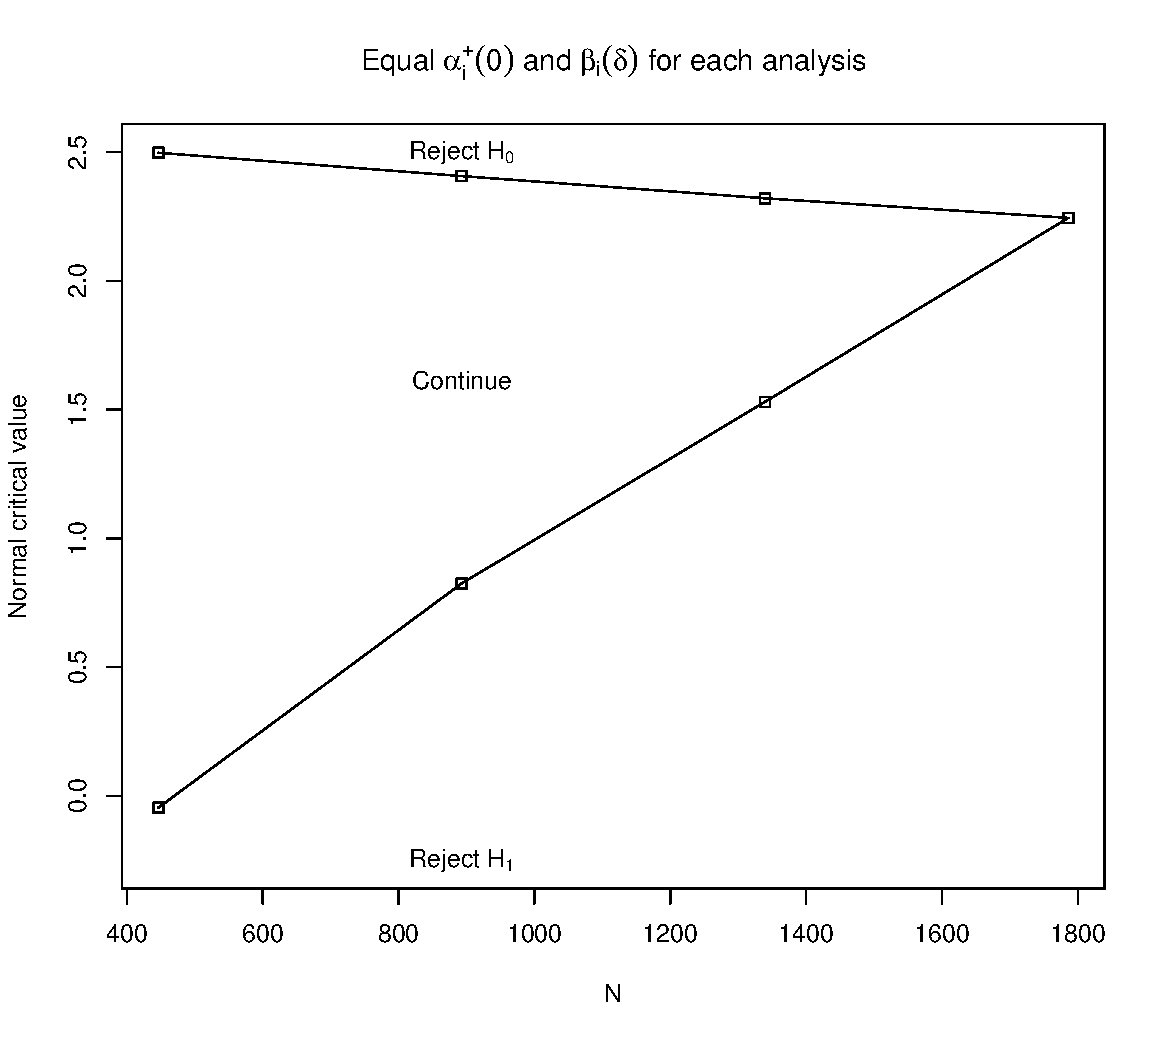
\includegraphics[width=.6\textwidth]{figs/boundplot2.pdf}
%RBC plot needs updating
\end{center}
\caption{Boundary plot for example 2}
\end{figure}%

\end{center}

O'Brien-Fleming, Pocock, or Wang-Tsiatis are normally used with equally-spaced
analyses. O'Brien-Fleming, Pocock, or Wang-Tsiatis (parameter of 0.4) bounds
for equally space analyses are generated as follows:

\bigskip

\begin{verbatim}
> xOF <- gsDesign(k=5, test.type=2, n.fix=1904, sfu="OF")
> xPk <- gsDesign(k=5, test.type=2, n.fix=1904, sfu="Pocock")
> xWT <- gsDesign(k=5, test.type=2, n.fix=1904, sfu="WT", sfupar=.4)
\end{verbatim}

\bigskip

Once you have generated these designs, examine the upper bounds as in 
Example~1.  Also, look at the spending by looking at, for example,
\texttt{xOF\$upper\$spend}.


\subsection*{Example 3: Logistic spending function}

Assume we would like the cumulative spending at 10\% of enrollment to be
$0.00125$ (5\% of total spending) and at 60\% of enrollment to be $0.005$ 
(20\% of total spending) so that $\alpha$-spending of $0.02$ is available for 
the final analysis; see \texttt{sfupar} in the following to find these 
numbers. This is the four-parameter specification of a logistic spending 
function (\texttt{sfLogistic()}, or the other two-parameter spending functions
\texttt{sfNormal()} and \texttt{sfCauchy()}). In each case, the four-parameter
specification is translated to the two essential parameters, but allows the
specification to be done simply.

\bigskip
\begin{verbatim}
> gsDesign(k=5, timing=c(.1, .25, .4, .6), test.type=2, n.fix=1904,
+ sfu=sfLogistic, sfupar=c(.1, .6, .05, .2))
Symmetric two-sided group sequential design with 90 % power and 2.5 % Type I Error.
Spending computations assume trial stops if a bound is crossed.

               
  Analysis   N   Z   Nominal p  Spend
         1  195 3.02    0.0013 0.0013
         2  488 3.04    0.0012 0.0011
         3  780 2.99    0.0014 0.0010
         4 1170 2.83    0.0023 0.0017
         5 1949 2.01    0.0223 0.0200
     Total                     0.0250 
++ alpha spending: Logistic spending function with a b = -1.629033 0.5986671

Boundary crossing probabilities and expected sample size assuming any cross stops the trial

Upper boundary (power or Type I Error)
          Analysis
   Theta      1      2      3      4     5 Total   E{N}
  0.0000 0.0013 0.0011 0.0010 0.0017 0.020 0.025 1936.1
  0.0743 0.0235 0.0686 0.1123 0.2077 0.488 0.900 1514.0

Lower boundary (futility or Type II Error)
          Analysis
   Theta      1      2     3      4    5 Total
  0.0000 0.0013 0.0011 0.001 0.0017 0.02 0.025
  0.0743 0.0000 0.0000 0.000 0.0000 0.00 0.000
\end{verbatim}
\bigskip

The same output can be obtained using the two-parameter specification of the
logistic spending function as follows (with values for \texttt{a} and 
\texttt{b} from above in \texttt{param}):

\bigskip

\begin{verbatim}
> y <- gsDesign(k=5, timing=c(.1, .25, .4, .6), test.type=2, n.fix=1904,
{+ sfu=sfogistic, sfupar=c(-1.629033, 0.5986671))
\end{verbatim}
\bigskip

To verify the initial spend is $0.00125$ (since it was rounded to 0.0013 above),
we examine the appropriate element of \texttt{y} just computed:

\bigskip

\begin{verbatim}
> y$upper$spend[1]
[1] 0.00125
\end{verbatim}


\subsection*{Example 4: gsProbability()}


We reconsider Example~1 and obtain the properties for the design for a larger
set of $\theta$ values than in the standard printout for \texttt{gsDesign()}.
The standard plot design for a \texttt{gsProbability} object is the power plot 
shown in Example~1. The boundary plot is obtainable below using the command
\texttt{plot(y, plottype=1)}.

\bigskip

\begin{verbatim}
> x <- gsDesign()
> y <- gsProbability(theta=x$delta*seq(0, 2, .25), d=x)
> y 
Asymmetric two-sided group sequential design with 90 % power and 2.5 % Type I Error.
Upper bound spending computations assume trial continues if lower bound is crossed.

           Sample
            Size    ----Lower bounds----  ----Upper bounds-----
  Analysis Ratio*   Z   Nominal p Spend+  Z   Nominal p Spend++
         1  0.357 -0.24    0.4057 0.0148 3.01    0.0013  0.0013
         2  0.713  0.94    0.8267 0.0289 2.55    0.0054  0.0049
         3  1.070  2.00    0.9772 0.0563 2.00    0.0228  0.0188
     Total                        0.1000                 0.0250 
+ lower bound beta spending (under H1): Hwang-Shih-DeCani spending function with gamma = -2
++ alpha spending: Hwang-Shih-DeCani spending function with gamma = -4
* Sample size ratio compared to fixed non-group sequential design

Boundary crossing probabilities and expected sample size assuming any cross stops the trial

Upper boundary (power or Type I Error)
          Analysis
   Theta      1      2      3  Total   E{N}
  0.0000 0.0013 0.0049 0.0171 0.0233 0.6249
  0.8104 0.0058 0.0279 0.0872 0.1209 0.7523
  1.6208 0.0205 0.1038 0.2393 0.3636 0.8520
  2.4311 0.0595 0.2579 0.3636 0.6810 0.8668
  3.2415 0.1412 0.4403 0.3185 0.9000 0.7913
  4.0519 0.2773 0.5353 0.1684 0.9810 0.6765
  4.8623 0.4574 0.4844 0.0559 0.9976 0.5701
  5.6727 0.6469 0.3410 0.0119 0.9998 0.4868
  6.4830 0.8053 0.1930 0.0016 1.0000 0.4266

Lower boundary (futility or Type II Error)
          Analysis
   Theta      1      2      3  Total
  0.0000 0.4057 0.4290 0.1420 0.9767
  0.8104 0.2349 0.3812 0.2630 0.8791
  1.6208 0.1138 0.2385 0.2841 0.6364
  2.4311 0.0455 0.1017 0.1718 0.3190
  3.2415 0.0148 0.0289 0.0563 0.1000
  4.0519 0.0039 0.0054 0.0097 0.0190
  4.8623 0.0008 0.0006 0.0009 0.0024
  5.6727 0.0001 0.0001 0.0000 0.0002
  6.4830 0.0000 0.0000 0.0000 0.0000
\end{verbatim}

\subsection*{Example 5: Non-inferiority testing }

We consider a trial examining a new drug that is more convenient to administer
than an approved control. There is no expectation of a substantially improved
response with the new drug. While the new drug may be a little better or
worse than control, there is some suggestion that the new drug may not be as
efficacious as control. Rather than powering the trial to show non-inferiority
when the new drug is slightly worse than control, the strategy is taken to
stop the trial early for futility if there is a `substantial' trend towards
the new drug being inferior. The control drug has provided a (binomial)
response rate of 67.7\% in a past trial and regulators have agreed with a
non-inferiority margin of 7\%. Let the underlying event rate in the control
and experimental groups be denoted by $p_{C}$ and $p_{E}$, respectively. Let
$\delta = 0.07$ represent the non-inferiority margin. There is no desire to stop
the trial early to establish non-inferiority. That is, this is a one-sided
testing problem for interim analyses. We let H$_{0}$: $p_{C}-p_{A}\leq0$ and
test against the alternative H$_{1}$: $p_{C}-p_{A}\geq\delta$., only stopping
early if H$_{0}$ can be rejected.\ We must have 97.5\% power to reject H$_{0}$
when H$_{1}$ is true ($\beta=0.025$) and can have a 10\% chance of rejecting
H$_{0}$ when H$_{0}$ is true ($\alpha=0.1$). In this case, an aggressive
stopping boundary is desirable to stop the trial 40\% of the way through
enrollment if the experimental drug is, in fact, not as efficacious as
control. The routine \texttt{FarrMannSS()} included with this package uses the
method of Farrington and Manning \cite{FarringtonManning}\ to compute the sample
size for a two-arm binomial trial for superiority or non-inferiority; see the
help file for documentation. As shown below, this requires 1966 patients for a
trial with no interim analysis; both nQuery and PASS2005 also yield this
result. Using this fixed sample size as input to \texttt{gsDesign()} yields a
sample size of 2332 for the trial compared to 2333 from EAST\ 5.2. This design
requires less than approximately a 4.5\% difference in event rates at the
interim analysis to continue and a final difference of no more than
approximately 3.3\% to achieve non-inferiority. These differences were
carefully evaluated in choosing the appropriate value of \texttt{gamma} for
the spending function.

\bigskip

\begin{verbatim}
> n.fix <- FarrMannSS(p1=.607, p2=.677, alpha=.1, beta=.025, sided=1, outtype=1)
> n.fix
[1] 1965.059
> gsDesign(k=2, alpha=.1, beta=.025, n.fix=n.fix, test.type=1, sfupar=3, timing=.4)
One-sided group sequential design with 97.5 % power and 10 % Type I Error.
               
  Analysis   N   Z   Nominal p  Spend
         1  933 1.45    0.0735 0.0735
         2 2332 1.68    0.0468 0.0265
     Total                     0.1000 
++ alpha spending: Hwang-Shih-DeCani spending function with gamma = 3

Boundary crossing probabilities and expected sample size assuming any cross stops the trial

Upper boundary (power or Type I Error)
          Analysis
   Theta      1      2 Total   E{N}
  0.0000 0.0735 0.0265 0.100 2228.7
  0.0731 0.7832 0.1918 0.975 1235.8
\end{verbatim}

\subsection*{Example 6: Non-inferiority and superiority testing in the same trial }


We consider a safety trial where a drug is given chronically to patients who
are expected to have a 3.5\% annual risk (exponential parameter $\lambda
_{0}=-\ln(1-0.035)=0.035627$) of developing cardiovascular disease (CVD) and
we wish to rule out an elevated risk that would be indicated by a hazard ratio
of 1.2 ($\lambda_{1}=1.2\lambda_{0}=0.042753)$. The desire is that if there is
a hazard ratio of 1.2 that there is at most a 2.5\% chance of demonstrating
non-inferiority. On the other hand, if the true hazard ratio is 1 (no excess
risk), we wish to have a 90\% probability of showing `no disadvantage'
(that is, we wish to rule out $\lambda_{1}\geq1.2\lambda_{0}$). In
hypothesis testing terms, the role of the null hypothesis (no difference) and
alternative hypothesis (20\% increased hazard ratio) have been reversed. We
label the hypotheses as before, but the error levels are reversed to
satisfy the above. We let the null hypothesis of no difference be denoted by
H$_{0}$: $\log(\lambda_{1}/\lambda_{0})=0$ and the alternate hypothesis is denoted by H$_{1}$: $\log(\lambda_{1}/\lambda_{0})=\log(1.2).$ To achieve
the desired performance, Type I error is set to 10\% and Type II error is set
to 2.5\%. Assume the trial is to be enrolled in a 2-year period and the
dropout rate is 15\% per year ($\lambda_{D}=-\ln(1-0.15)=0.162519$). As seen
below, fixed design with no interim analysis requires a sample size of 6,386
per treatment group to obtain 1,570 total events (under in 6 years H$_{1}$).
Note that under the null hypothesis, the overall event rate would be lower and
it would take longer to obtain the number of events required.

\bigskip
\begin{verbatim}
> # exponential control group failure rate of 3.5 percent per year
> lambda.0 <- -log(1-.035)
> # wish to rule out experimental group hazard ratio of 1.2 
> lambda.1 <- 1.2*lambda.0
> # dropout rate of 15 percent per year
> eta <-  -log(1-.15)
> # fixed design sample size
> # recruitment time Tr=2 years, total study time Ts=6 years
> SSFix <-nSurvival(lambda.0=lambda.0, lambda.1=lambda.1, eta=eta, alpha=.1, beta=.025,
+ type="rr", Ts=6, Tr=2)
> # show sample size per group and total number of events required for fixed design
> ceiling(SSFix$Sample.size/2)
[1] 6386
> ceiling(SSFix$Num.events)
[1] 1570
\end{verbatim}
\bigskip

We use the above sample size and number of events below to adjust this
fixed design to a group sequential design and obtain the number of events
required at each analysis. In addition, we consider the possibility that the
experimental drug may actually reduce cardiovascular risk. For a fixed design,
superiority testing may be performed following non-inferiority testing. For a
group sequential trial, the situation is slightly more complex; this is not a
scenario that can be dealt with in EAST 5.2. We take two approaches to this.
First, we consider non-inferiority of control to treatment to be of no
interest, which leads to an asymmetric design. Second, we consider the problem
to be symmetric: inference on one arm relative to the other uses identical
criteria; this will be deferred to example 7
%RBC: there is currently no example 7

Let H$_{0}$: $\theta = 0$ and H$_{1}$: $\theta\neq0$ where $\theta$ indicates
the underlying difference between two treatment groups. We wish to show that a
new treatment is non-inferior compared to control. That is, for some
$\delta > 0,$ under H$_{1A}$: $\theta = \delta$ we wish to have 97.5\% power to
reject H$_{0}$: $\theta = 0$ (i.e., \texttt{beta=0.025} to yield a 2.5\% chance
of accepting non-inferiority when in fact the underlying effect for the
experimental group is higher by $\delta$). On the other hand, under H$_{0}$:
$\theta=0$ we are willing to have a 10\% chance of rejecting H$_{0} $:
$\theta=0$ in favor of H$_{1A}$: $\theta=\delta$ (\texttt{alpha=0.10} to yield
90\% power to show non-inferiority). We have a slightly asymmetric test for
superiority in that we would like to reject H$_{0}$: $\theta$=0 in favor of
H$_{1B}$: $\theta=-\delta$ at the 2.5\% (one-sided) level 
(\texttt{astar=0.025}) to control Type I error in that direction. Thus, 
the trial could stop early if $\theta$ is substantially different from $0$ 
in either direction. A Hwang-Shih-DeCani spending function with 
\texttt{sfupar=sflpar=-4} is used for
each bound. The bounds are asymmetric due to the different levels of the test
in each direction. The appropriate confidence interval approach for this
design is probably a stage-wise ordering approach (see Jennison \& Turnbull
\cite{JTBook}, sections 8.4 and 8.5). This gives the tightest intervals at
the end of the trial and does not result in conflicts between the confidence
intervals and the testing approach just outlined.

See output below for a design with four equally spaced interims. With
\texttt{n.fix=1264} we find that $\delta=0.0818$. Interestingly, there is
90\% power to cross the lower bound under H$_{1B}$: $\theta = -\delta$, so the
trial is well-powered for superiority of the experimental treatment. The
design requires an increase from 1570 events to 1595 in order to maintain the
desired error rates with the given stopping rules. Note that
\texttt{test.type=5} indicates that all bounds are binding and both upper and
lower bound error spending is under the null hypothesis. The upper bound is a
futility bound for showing non-inferiority. If it is never crossed, the trial
establishes non-inferiority. The lower bound is the superiority bound.

\bigskip
\begin{verbatim}
> # show number of events required at interim and final analysis
> # of group sequential design
> x <- gsDesign(test.type=5, k=5, alpha=.1, beta=.025, astar=.025, sflpar=-4,
+               sfupar=-4, n.fix=SSFix$Num.events)
>
> # show sample size per group required using same inflation factor as
> # for number of events
> ceiling(x$n.I[5]/SSFix$Num.events*SSFix$Sample.size/2)}
[1] 6491
>
> # show power at + or - delta and 0
> y <- gsProbability(d=x, theta=c(-x$delta, 0, x$delta))
> y
Asymmetric two-sided group sequential design with 97.5 % power and 10 % Type I Error.
Spending computations assume trial stops if a bound is crossed.

                  ----Lower bounds----  ----Upper bounds-----
  Analysis   N    Z   Nominal p Spend+  Z   Nominal p Spend++
         1  319 -3.25    0.0006 0.0006 2.84    0.0023  0.0023
         2  638 -2.99    0.0014 0.0013 2.52    0.0059  0.0051
         3  957 -2.69    0.0036 0.0028 2.17    0.0150  0.0113
         4 1276 -2.37    0.0088 0.0063 1.78    0.0376  0.0252
         5 1595 -2.03    0.0214 0.0140 1.33    0.0916  0.0561
     Total                      0.0250                 0.1000 
+ lower bound spending (under H0): Hwang-Shih-DeCani spending function with gamma = -4
++ alpha spending: Hwang-Shih-DeCani spending function with gamma = -4

Boundary crossing probabilities and expected sample size assuming any cross stops the trial

Upper boundary (power or Type I Error)
          Analysis
    Theta      1      2      3      4      5 Total   E{N}
  -0.0818 0.0000 0.0000 0.0000 0.0000 0.0000 0.000 1150.8
   0.0000 0.0023 0.0051 0.0113 0.0252 0.0561 0.100 1566.1
   0.0818 0.0847 0.2516 0.3181 0.2255 0.0951 0.975  971.2

Lower boundary (futility or Type II Error)
          Analysis
    Theta      1      2      3      4      5 Total
  -0.0818 0.0366 0.1497 0.2632 0.2700 0.1785 0.898
   0.0000 0.0006 0.0013 0.0028 0.0063 0.0140 0.025
   0.0818 0.0000 0.0000 0.0000 0.0000 0.0000 0.000
> plot(y, plottype="xbar")
\end{verbatim}
\bigskip

The plot below shows the cumulative probabilities of stopping at each analysis
for different values of $\theta$. The solid lines go from the probability of
stopping at the first interim analysis to the highest line which shows the
probability of an inferiority finding at any analysis. The dashed lines
provide 1 minus the cumulative probability of stopping for superiority for
different values of $\theta$ for each analysis. Note that the expected sample
size required to come to a conclusion if the experimental regiment is truly
inferior to control (H$_{1A}$: $\theta = \delta$) is 653 events compared to 1264
for a fixed design. In addition, there is only a 6.8\% chance of continuing
the trial to the final analysis. This is comprised of a 2.5\% of continuing
the trial to the final analysis and falsely establishing non-inferiority plus a
4.27\% of continuing to the trial to the final analysis to establish
inferiority. If experimental therapy is truly superior, the expected number of
events required to demonstrate a difference is 950. If there is truly no
difference the trial usually goes to the end (about 91\% of the time; this is
seen by the last result below) and finds no difference (87.5\% of the time;
this is the sum of the Type I error in both directions).

Evaluation of the cutoffs has not been performed as in Example 5. This
exercise would be worthwhile to verify that the cutoffs of the design are appropriate.

\bigskip
\begin{verbatim}
> x <- gsDesign(test.type=5, k=5, alpha=.1, beta=.025, astar=.025, sflpar=-3,
+ sfupar=0, n.fix=1264)
> y <- gsProbability(d=x, theta=c(-x$delta, 0, x$delta))
> y
Asymmetric two-sided group sequential design with 97.5 % power and 10 % Type I Error.
Spending computations assume trial stops if a bound is crossed.

                  ----Lower bounds----  ----Upper bounds-----
  Analysis   N    Z   Nominal p Spend+  Z   Nominal p Spend++
         1  284 -3.07    0.0011 0.0011 2.05    0.0200    0.02
         2  567 -2.84    0.0022 0.0020 1.91    0.0278    0.02
         3  850 -2.60    0.0047 0.0036 1.79    0.0368    0.02
         4 1133 -2.34    0.0097 0.0065 1.68    0.0465    0.02
         5 1417 -2.06    0.0197 0.0119 1.58    0.0568    0.02
     Total                      0.0250                 0.1000 
+ lower bound spending (under H0): Hwang-Shih-DeCani spending function with gamma = -3
++ alpha spending: Hwang-Shih-DeCani spending function with gamma = 0

Boundary crossing probabilities and expected sample size assuming any cross stops the trial

Upper boundary (power or Type I Error)
          Analysis
    Theta      1     2      3      4      5  Total   E{N}
  -0.0912 0.0002 0.000 0.0000 0.0000 0.0000 0.0002  950.0
   0.0000 0.0200 0.020 0.0200 0.0200 0.0200 0.1000 1352.8
   0.0912 0.3018 0.325 0.2048 0.1007 0.0427 0.9750  653.6

Lower boundary (futility or Type II Error)
          Analysis
    Theta      1      2      3      4      5  Total
  -0.0912 0.0625 0.1988 0.2796 0.2396 0.1401 0.9207
   0.0000 0.0011 0.0020 0.0036 0.0065 0.0119 0.0250
   0.0912 0.0000 0.0000 0.0000 0.0000 0.0000 0.0000
> plot(gsProbability(k=5, n.I=x$n.I, a=x$lower$bound, b=x$upper$bound,
+ theta=x$delta*(-25:25)/25))
> # compute probability of continuing to the end of the trial under H0
> 1-sum(y$upper$prob[1:4, 2] + y$lower$prob[1:4, 2])
[1] 0.9068707
\end{verbatim}

\begin{center}%
\begin{figure}
\begin{center}
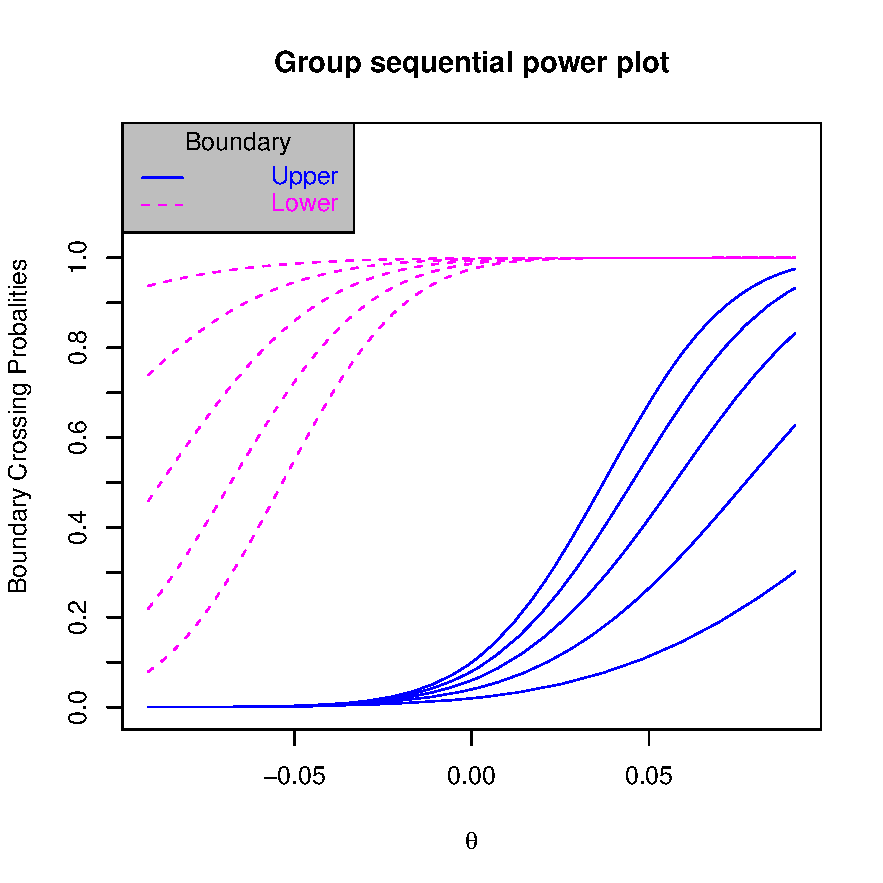
\includegraphics[width=.6\textwidth]{figs/noninferiority.pdf}
\end{center}
\caption{Power plot for non-inferiority design in example 6}
\end{figure}%

\end{center}

